OpenID standardin ensimmäisen version kehitti toukokuussa 2005 Brad Fitzpatrick \cite{openid}. Tuoreimman (2.0) version kehitys aloitettiin 2007 ja se on edelleen aktiivista. OpenID on SAML:ia rajoitetumpi protokolla, koska se tarjoaa vain käyttäjän tunnistautumisen. Sen tavoite on saman käyttäjätunnuksen käytön mahdollistaminen eri web-sovelluksissa. Nykyään sen kehityksestä vastaa \mbox{OpenID} Foundation -säätiö, jonka jäseniä ovat mm. Faceobok, Google ja Microsoft \cite{openid_foundation}.

OpenID-palveluntarjoaja tarjoaa päätepisteen (endpoint), jota web-sovellukset käyttävät tunnistautumiseen. Tunnistautumiseen voidaan käyttää kahta erilaista tapausta (flow). Suunnatussa identiteetin (directed identity) tapauksessa käyttäjä valitsee palveluntarjoajan, jonka kautta kirjautuminen suoritetaan \cite{openid}. Väitetyn identiteetin (claimed identity) tapauksessa web-sovellus hakee päätepisteen annetun \mbox{OpenID}\--tun\-nis\-teen perusteella \cite{openid}. Tapaukset eroavat toisistaan vain vaiheessa, jossa etsitään päätepiste. Kuvassa \ref{openid_flow} on esitetty OpenID-kirjautumisen vaiheet.

\begin{figure}[ht]
\centering
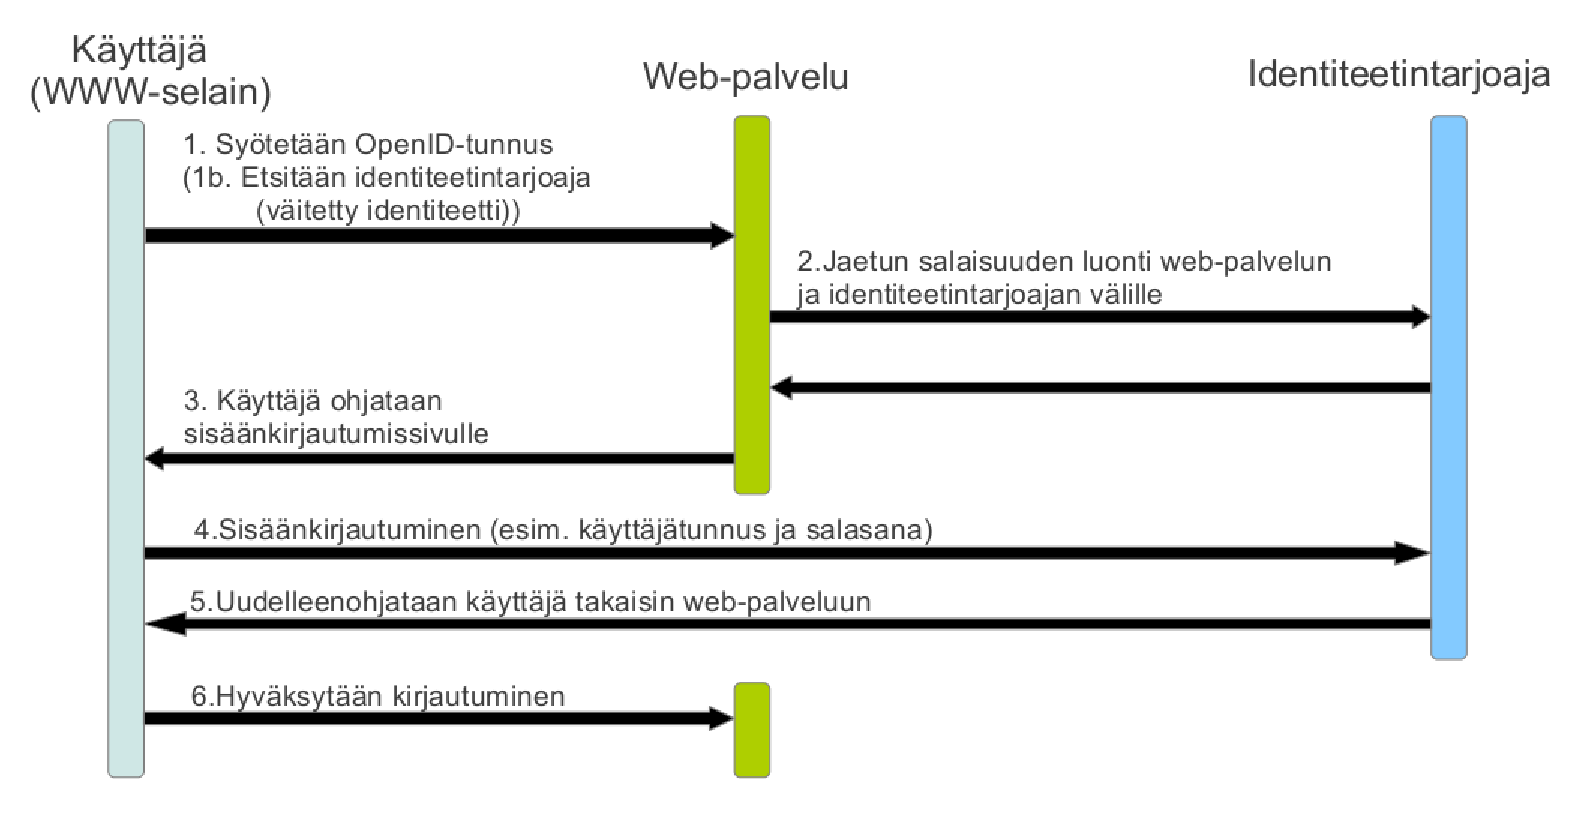
\includegraphics[width=\textwidth]{teknologiat/protokollat/openid.eps}
\caption{OpenID-kirjautumisen vaiheet \cite{openid}.}%
\label{openid_flow}
\end{figure}

OpenID:n suhteen odotukset olivat alkujaan suuria, mutta myöhemmin into on laantunut. Esimerkiksi Microsoftin vuonna 2008 aloittama OpenID-kokeilu lopetettiin elokuussa 2009, minkä jälkeen Microsoft on siirtynyt käyttämään omaa tunnistautumistoteutusta \cite{openid_microsoft}. OpenID-protokollaan liittyvät turvallisuushuolet ovat kasvaneet viime aikoina, koska se koetaan alttiiksi erilaisille kalasteluhyökkäyksille \cite{billion_keys}.

Julkisen Internetin puolella yleiset OpenID-kir\-jau\-tu\-mis\-si\-vut on korvattu lähes kokonaan eri palveluntarjoajien omilla kirjautumissivuilla. Käyttäjätutkimusten mukaan käyttäjät eivät tunne OpenID:tä, mutta tuntevat palveluntarjoajan kuten Googlen tai Yahoon \cite{refuse_sso}. Näin ollen käyttäjät eivät koe kirjautuvansa OpenID:llä palveluun, johon kirjaudutaan Googlen tunnuksilla. Myös alkuperäinen ajatus siitä, että kuka tahansa voi toimia identiteetintarjoajana, on osoittautunut toimimattomaksi, koska web-sovellusten ylläpitäjät haluavat luottaa päätepisteisiin, joiden kautta heidän palveluunsa voi kirjautua \cite{refuse_sso}. Tämän vuoksi rajoitetumpaan käyttöön soveltuvat protokollat, kuten OAuth, ovat kasvattaneet suosiotaan.

Standardiin liittyvien ongelmien ja rajoitusten löytymisen jälkeen on käynyt selväksi, että \mbox{OpenID:n} kehitystyötä täytyy jatkaa. Yksi OpenID:n keskeinen rajoitus on, että se varmistaa vain käyttäjän olevan se, joka väittää olevansa, mutta se ei ota kantaa käyttäjän pääsyoikeuksiin. Laajentaakseen protokollaa OpenID-säätiö on julkaisemassa uuden OpenID Connect -määritelmän, joka lisää protokollaan myös pääsynvalvonnan \cite{distributed_web_security}. Sen kehitys on kuitenkin vielä niin varhaisessa vaiheessa, että sen tutkiminen tämän tutkielman puitteissa ei ole mielekästä.